\chapter{Schritt 5 neu}
\label{chap:Schritt-5}

Im letzten Schritt wurde das primäre Problem der Formularanwendung gelöst:
Auswahloptionen sollen nur dann anwählbar sein,
wenn sie die ihr hinterlegte Bedingung erfüllen.
Darüber hinaus können nur Maßnahmen gespeichert werden,
deren Auswahloptionen untereinander kompatibel sind.

Durch das Lösen dieses Problems ist ein neues Problem entstanden:
Alle Selektionskarten müssen bei einer Selektion neu gezeichnet werden.
Dieses Verhalten kann auch bei Ausführung der Applikation im Debugmodus in \enquote{Android Studio} beobachtet werden.
Der \enquote{Flutter Performance}-Tab gibt eine Übersicht über die Anzahl der im letzten \enquote{Frame} neu gezeichneten \enquote{Widgets}. 
Dieser zeigt, dass sich bei jeder Auswahl einer Option sechs \enquote{Card}-Elemente aktualisieren \Abb{\ref{fig:Schritt5_6rebuilds}}.
Das ist der Fall, da es im Formular in Summe sechs Selektionskarten mit einem darin befindlichen \enquote{Card}-Widget gibt.

\begin{figure}[ht]
  \centering
  \ifIncludeFigures
  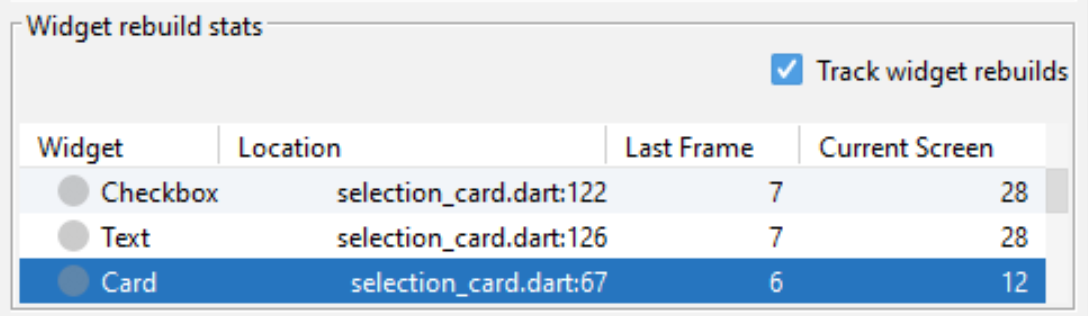
\includegraphics[width=0.8\textwidth]{Inhalt/Hauptteil/Implementierung/Schritt-5/6rebuilds.png}
  \fi
  \caption[Das \enquote{Card}-\enquote{Widget} wird sechsmal neu gezeichnet]{Das \enquote{Card}-\enquote{Widget} wird sechsmal neu gezeichnet, Quelle: Eigene Abbildung}
  
  \label{fig:Schritt5_6rebuilds}
\end{figure}%


Bei einer geringen Anzahl von Auswahlfeldern sollte das noch keine gravierenden Auswirkungen auf das Laufzeitverhalten der Applikation haben.
Doch je zahlreicher die Auswahlfelder werden,
desto länger dauert die Aktualisierung der Oberfläche.

Das Problem kann folgendermaßen entschärft werden:
Noch bevor das \enquote{Widget} \IC{SelectionCard} den \IC{StreamBuilder} in der \IC{build}-Methode zurückgibt,
wird der \enquote{Stream} \IC{validityChanged} erstellt \LstSZ{lst:Schritt5needsRepaint}{51-54}.

Es handelt sich um eine sogenannte Transformation des \enquote{Streams} \IC{priorChoices}, welcher die Momentaufnahme aller ausgewählten Optionen im gesamten Formular übermittelt.
Immer dann, wenn der \enquote{Stream} \IC{priorChoices} ein neues Ereignis sendet,
geschieht für die Abwandlung dieses \enquote{Streams} folgendes:
Die Methode \IC{map} wandelt jedes Ereignis in ein neues Objekt um \Z{52}.
Die aktuelle Momentaufnahme der Auswahloptionen im Formular wird dazu im Parameter \IC{choices} gespeichert.
Bei der Umwandlung des Ereignisses werden die ausgewählten Optionen der aktuellen Selektionskarte über \IC{selectionViewModel.value} abgerufen \Z{53}.
Sollte es sich beispielsweise bei der aktuellen Selektionskarte um das Auswahlfeld der \enquote{Zieleinheit} handeln,
so könnte der ausgewählte Wert \enquote{ha} sein.

Mit dem Aufruf \IC{.any((c) => !c.conditionMatches(choices))} wird nun überprüft, ob der ausgewählte Wert
-- im Fall eines Einfachauswahlfeldes --
oder die ausgewählten Werte
-- bei einem Mehrfachauswahlfeld --
mit der neuen Momentaufnahme der Selektionen im Formular kompatibel sind.
Für die \enquote{Zieleinheit} \enquote{ha} gelten folgenden Bedingungen:
Für die \enquote{Zielfläche} dürfen die Option \enquote{keine Angabe/Vorgabe} und
\enquote{bitte um Unterstützung} nicht gewählt sein \LstZ{\ref{lst:Schritt5ha}}{166-167}.
Das bedeutet im Umkehrschluss,
dass nur die Optionen \enquote{AL},
\enquote{GL},
\enquote{LF},
\enquote{DK/SK},
\enquote{HFF},
\enquote{Landschaftselement/Biotop o.Ä.} 
oder \enquote{Wald/Forst} gewählt sein dürfen. 

\begin{alexlisting}{Schritt 4}{Der Klassenvariable \enquote{ha} des Typs \enquote{ZielflaecheChoice} wird eine Bedingung hinzugefügt}
  {Quellcode/Schritt-5/conditional_form/lib/choices/choices.dart}
  {firstline=164, lastline=167}
  \label{lst:Schritt5ha}
\end{alexlisting}

Wurde also beispielsweise bei der neuen Selektion in der \enquote{Zielfläche} die Option \enquote{keine Angabe/Vorgabe} ausgewählt,
so würde die Option \enquote{ha} invalide werden,
da sie nicht mit den \enquote{Zieleinheit}-Optionen \enquote{keine Angabe/Vorgabe} bzw. \enquote{bitte um Unterstützung}  kompatibel ist.

Die Methode \IC{map} \LstSZ{lst:Schritt5needsRepaint}{52} wandelt also das neue Ereignis der Momentaufnahme aller Selektionen im Formular in einen einzigen Wahrheitswert um.
Ist der Wahrheitswert \IC{true},
bedeutet dies,
dass alle ausgewählten Optionen in der aktuellen Selektionskarte valide sind.
Ist er dagegen \IC{false}, so ist wenigstens eine der Auswahloptionen mit den restlichen Selektionen der anderen Auswahlfelder im Formular inkompatibel.



Der resultierende \enquote{Stream} wird weiter transformiert: Durch die Funktion \IC{distinct} \Z{54} werden nur Ereignisse gesendet,
sofern sie sich von dem letzten Ereignis unterscheiden.
Der \enquote{Stream} \IC{validityChanged} sendet also immer genau dann Ereignisse,
wenn sich etwas an der Validität der Auswahloptionen der aktuellen Selektionskarte ändert.

\begin{alexlisting}{Schritt 5}{Der \enquote{Stream} \enquote{validityChanged} in Schritt 5}
  {Quellcode/Schritt-5/conditional_form/lib/widgets/selection_card.dart}
  {firstline=51, lastline=71, highlightlines={51-58,61}}
  \label{lst:Schritt5needsRepaint}
\end{alexlisting} 

Doch dieser \enquote{Stream} kann nicht für den \IC{StreamBuilder} benutzt werden.
Denn wenn sich die Auswahl in der aktuellen Selektionskarte ändert
und die Validität dadurch unverändert bleibt,
so erfolgt kein neues Zeichnen der Selektionskarte.
Es muss aber eine Aktualisierung stattfinden, damit der neue Wert in der Selektionskarte abgebildet wird.
Deshalb ist eine Kombination der \enquote{Streams} \IC{validityChanged} und \IC{selectionViewModel} erforderlich.
Das \IC{BehaviorSubject} \IC{needsRepaint} soll als diese Kombination fungieren \Z{56}.
Es wird mit dem Wert \IC{true} initialisiert.
Dafür ist unerheblich, welcher Wert in dem \enquote{Stream} aktuell gespeichert ist. \pdfcomment[icon=Note,color=yellow]{27.08.2021 Dieser Satz wurde angepasst}
Lediglich dass ein neues Ereignis hinzugefügt wird,
um die Aktualisierung der Oberfläche auszulösen,
ist wesentlich.
Mit der Methode \IC{listen} wird nun sowohl auf den \enquote{Stream} \IC{validityChanged} \Z{57} als auch auf \IC{selectionViewModel} \Z{58} gehorcht. 
Jedes empfangene Ereignis wird dabei dem \IC{BehaviorSubject} \IC{needsRepaint} hinzugefügt.
Dadurch,
dass \IC{needsRepaint} für den \IC{StreamBuilder} verwendet wird \Z{61},
zeichnet sich die Selektionskarte immer dann neu,
wenn sich die beinhaltenden Auswahloptionen oder aber deren Validität ändern.\pdfcomment[icon=Note,color=yellow]{27.08.2021 Dieser Satz wurde angepasst}


Ein Beispiel:
Für die \enquote{Zielfläche} ist \enquote{AL} und für die \enquote{Zieleinheit} ist \enquote{ha} ausgewählt.
Beide Optionen sind miteinander kompatibel.
Nun erfolg eine weitere Selektion.
Für \enquote{Zielfläche} wird nun die Option \enquote{GL} gewählt.
Auch sie ist mit der \enquote{Zieleinheit} \enquote{ha} kompatibel.
Durch die Selektion hat sich der Wert der Selektionskarte der \enquote{Zielfläche} geändert, weshalb sie neu gezeichnet werden muss.
Alle anderen Auswahlfelder im Formular sind nicht betroffen.
Im \enquote{Flutter Performance}-Tab ist zu beobachten,
dass das \enquote{Widget} \IC{Card} nur einmal neu gezeichnet wurde \Abb{\ref{fig:Schritt5_1rebuild}}.

\begin{figure}[ht]
  \centering
  \ifIncludeFigures
  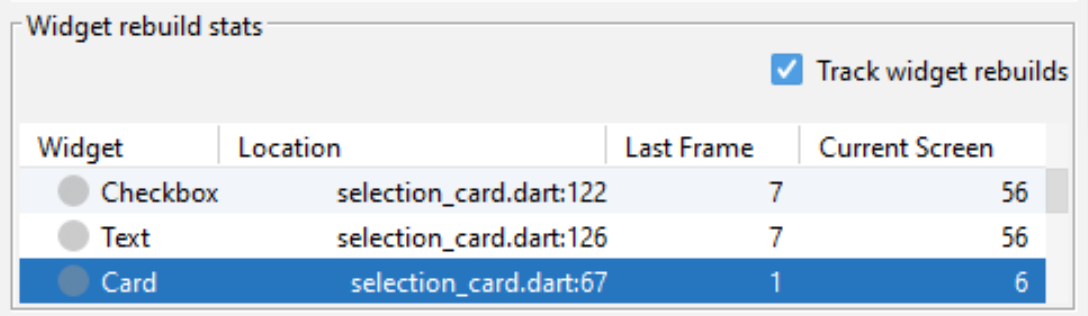
\includegraphics[width=0.8\textwidth]{Inhalt/Hauptteil/Implementierung/Schritt-5/1rebuild.png}
  \fi
  \caption[Das \enquote{Card}-\enquote{Widget} wird einmal neu gezeichnet]{Das \enquote{Card}-\enquote{Widget} wird einmal neu gezeichnet, Quelle: Eigene Abbildung}
  
  \label{fig:Schritt5_1rebuild}
\end{figure}%


Durch eine weitere Selektion für \enquote{Zielfläche} soll nun provoziert werden, dass die Auswahl der  \enquote{Zieleinheit} invalide wird.
Deshalb wird für die \enquote{Zielfläche} nun \enquote{keine Angabe/Vorgabe} selektiert.
Die \enquote{Zieleinheit} \enquote{ha} ist damit nicht kompatibel.
Deshalb müssen sich nun zwei Auswahlfelder aktualisieren:
\begin{itemize}[topsep=0pt,itemsep=-1ex,partopsep=1ex,parsep=1ex]
  \item die Selektionskarte \enquote{Zielfläche}, weil sich der darin ausgewählte Wert geändert hat und
  \item die Selektionskarte \enquote{Zieleinheit}, da sie zuvor valide war und nun invalide ist.
\end{itemize}

Der \enquote{Flutter Performance}-Tab reflektiert dies,
da sich das \enquote{Widget} \IC{Card} nun zweimal neu zeichnet \Abb{\ref{fig:Schritt5_2rebuilds}}.

\begin{figure}[ht]
  \centering
  \ifIncludeFigures
  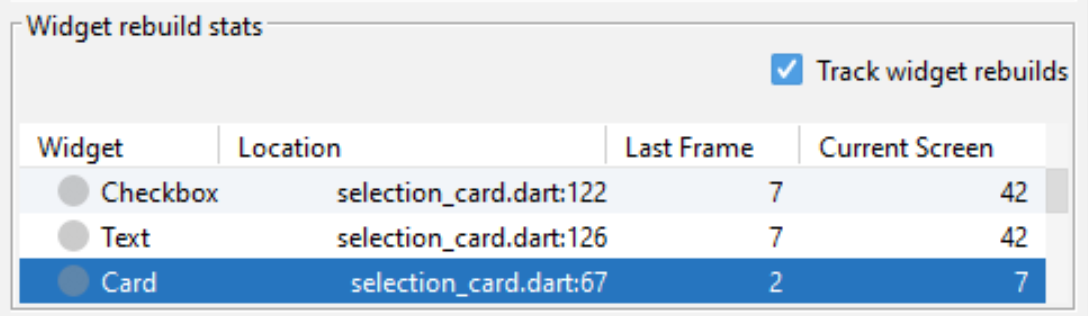
\includegraphics[width=0.8\textwidth]{Inhalt/Hauptteil/Implementierung/Schritt-5/2rebuilds.png}
  \fi
  \caption[Das \enquote{Card}-\enquote{Widget} wird zweimal neu gezeichnet]{Das \enquote{Card}-\enquote{Widget} wird zweimal neu gezeichnet, Quelle: Eigene Abbildung}
  
  \label{fig:Schritt5_2rebuilds}
\end{figure}%